%Exp 1-6
\chapter{Conservation of Momentum}
\label{chap:conservationofmomentum}
%\maketitle
\newcounter{saveenumerate}
\makeatletter
\newcommand{\enumeratext}[1]{%
\setcounter{saveenumerate}{\value{enum\romannumeral\the\@enumdepth}}
\end{enumerate}
#1
\begin{enumerate}
\setcounter{enum\romannumeral\the\@enumdepth}{\value{saveenumerate}}%
}
\makeatother

\section{Introduction}

Momentum is one of the central quantities in physics and, like energy, is bound by a conservation law in the absence of external forces. Although conservation of momentum is less intuitive to many people than conservation of energy, conservation of momentum can be applicable in situations where conservation of energy is not. Sometimes, conservation of energy may not be easily utilized since it can be difficult to keep track of all possible energy contributions (such as energy contribution that deforms the metal of two cars as they collide), but conservation of momentum may still be helpful. For some problems, momentum conservation is essential. We will see that specific problems, like the ballistic pendulum that you will study today, require both energy and momentum conservation for their solution. Others, like collisions on the airtrack, can be solved by momentum conservation where mechanical energy is conserved (elastic) as well as where mechanical energy is not conserved (inelastic). This lab is designed to expose you to several conservation of momentum examples to provide you with an intuitive sense of momentum and some of its important applications\footnote{See Chapter 9 of \emph{Fundamentals of Physics} by Halliday, Resnick \& Walker.}.\myskip

\underline{\emph{Remark}:} You must prepare some derivations (mainly for projectile velocity in the ballistic pendulum part) \underline{at home}; otherwise you may not finish the lab on time!

\section{Theory}
\subsection{Momentum Conservation}
Momentum is a vector quantity, so it has magnitude and direction. To add or subtract momenta, one must use the usual rules of vector addition (see lab \ref{chap:forces} "Forces"). In this lab, we deal only with momentum in one dimension, so the vector property is applicable only in the sense that if two objects move in opposite directions, their momenta have opposite signs. This is the source of most mistakes when performing calculations with momenta, so be careful. \myskip

Momentum is the product of mass and velocity:
\begin{equation}
\vec p=m \vec v
\end{equation}
A fundamental property of nature is that the total momentum components of any closed system\footnote{A closed system is one in which the sum of forces \underline{external} to the specified system is zero.} are conserved in any physical process {\it{in which external forces are absent}}.
\subsection{The Air Track}

Using the gliders on the air track, we will test momentum conservation by measuring momentum of the gliders before and after collisions. Since momentum is the product of mass and velocity, we simply need to measure the mass of the gliders using a balance, and measure the velocities using the apparatus we saw in the velocities lab. We are going to study two different kinds of collisions:\myskip

A). \textbf{Elastic Collision}. In the first experiment performed on the air track, two gliders with masses $m$ and $M$ will start with velocities $\vec v_{1i}$ and $\vec v_{2i}$. We will use the sonic ranger to measure these velocities following procedures described in section 3. After the collision, the velocities become $\vec v_{1f}$ and $\vec v_{2f}$. The gliders will undergo nearly perfectly elastic collision, so we can assume both energy and momentum are conserved:
\begin{align}
    m\vec v_{1i} + M\vec v_{2i} &=  m\vec v_{1f} + M\vec v_{2f} \\
    \frac{1}{2}mv_{1i}^2 + \frac{1}{2}Mv_{2i}^2 &= \frac{1}{2}mv_{1f}^2 + \frac{1}{2}Mv_{2f}^2
\end{align}
After some algebra, you should be able to solve $v_{1f}$ and $v_{2f}$ from the above two equations, and the result should be
\begin{equation}
   \vec  v_{1f} = \frac{2M \vec v_{2i} - (M-m)\vec v_{1i}}{M+m},\quad \vec v_{2f} = \frac{2m \vec v_{1i} + (M-m)\vec v_{2i}}{M+m}
  \label{eq:velocities}
\end{equation}
Note: you must make sure to use the correct sign in the expressions for $v_{1f}$ and $v_{2f}$ since velocities are vectors. Be careful when interpreting the graphs on DataStudios since both Sonic Rangers will read positive velocities even though the carts travel in opposite directions (you will have to interpret one Ranger as measuring positive velocities and the other as measuring negative velocities).
\\
\\
A special case of the above equations is when the two masses are equal, $M=m$, the equations can be simpified into
\begin{equation}
  \vec  v_{1f} = \vec v_{2i},\quad \vec v_{2f} = \vec v_{1i}
\end{equation}
or in other words, the two gliders just exchange their velocities.
\myskip

B). \textbf{Inelastic Collision}. In the second experiment the two gliders will stick together after collision. This is called a perfectly inelastic collision meaning that the kinetic energy is no longer conserved. Momentum, however, is still conserved in this case and, because the two gliders stick together after collision, there is only one unknown final velocity. The momentum conservation equation reads
\begin{equation}
    m\vec v_{1i} + M\vec v_{2i} = (m+M)\vec v_f
\end{equation}
where $\vec v_f$ is the common final velocity of the two gliders.

\subsection{The Ballistic Pendulum}

A ballistic pendulum is an instrument usually used to indirectly measure the velocity of a projectile. A fast metal ball strikes a stationary pendulum (in our case a small cup with a latch on the top) and sticks to it. The initial velocity of the ball can be deduced by observing how far the pendulum swings after the collision. In this experiment, we will measure angular displacement of the pendulum, and use that value to estimate the metal ball's initial velocity. We can then compare the measurement with the pre-measured velocity data. % We can then compare our estimated initial velocity to the velocity we measure with a sensitive photogate timing system.\myskip

To analyze this problem, it is easiest to start by splitting it into two parts. In the first part, consider the metal ball and pendulum in the time right before and right after the collision. The pendulum is initially at rest at its equilibrium point, whereas the metal ball travels with an initial velocity and therefore nonzero kinetic energy. When the ball strikes the pendulum, they stick together and move at the same velocity. But because an unknown part of the initial kinetic energy is lost via vibrations, we cannot directly calculate the pendulum's subsequent motion from conservation of mechanical energy.  Instead, we can use conservation of momentum, since during the small time of the collision there are no external forces acting in the direction of motion.\myskip

Quantitatively, consider the ball to have a mass $m$ and initial velocity $\vec v$, and the pendulum to have a mass $M$ (concentrated completely at the pendulum's end) and initial velocity of 0. The total initial momentum is $mv$. When the projectile and the pendulum stick together, they have total mass $m + M$ and we define their combined velocity to be $\vec V$. The relationship from conservation of momentum is:
\begin{equation}
    m \vec v = (m+M)\vec V
\end{equation}
So if we know the initial velocity of the projectile $\vec v$, we can calculate the combined velocity of the projectile and pendulum $\vec V$.\myskip

\begin{figure}[h]
    \begin{center}
        \begin{tikzpicture}
            \begin{scope}[dashed]
                \draw (0,0) rectangle (0.2,4);
                \draw (-0.4,0) rectangle (0.6,-1);
                \draw (-0.4,-1) rectangle (-0.1,-1.5);
                \draw (0.6,-1) rectangle (0.3,-1.5);
                \draw (-0.1,-1) rectangle (0.3,-1.2);
                \draw (-0.1,-1.2) rectangle (0.3,-1.4);
                \draw[dashed] (0.1,-0.5) circle (0.3);
            \end{scope}

            \begin{scope}[rotate around={35:(0.1,4)}]
                \draw (0,0) rectangle (0.2,4);
                \draw (-0.4,0) rectangle (0.6,-1);
                \draw (-0.4,-1) rectangle (-0.1,-1.5);
                \draw (0.6,-1) rectangle (0.3,-1.5);
                \draw (-0.1,-1) rectangle (0.3,-1.2);
                \draw (-0.1,-1.2) rectangle (0.3,-1.4);
                \draw[dashed] (0.1,-0.5) circle (0.3);

                \draw[dashed] (0.1,4) -- (1.6,4);
                \draw[dashed] (0.1,-0.5) -- (1.6,-0.5);
                \draw[>=stealth,<->,thick] (1.4,-0.5) -- node[right] {$R$} (1.4,4);
                \node (A) at (0.1,-0.5) {};
            \end{scope}
            \draw[xshift=-2cm] (0.1,-0.5) circle (0.3);
            \draw[>=triangle 60,->,xshift=-2cm] (-0.5,-1.2) --  node[below] {$v$}(0.5,-1.2);

            \draw[>=stealth,<->,thick] (0.2,2.5) arc (-85:-58:1.5cm);
            \node at (0.7,2.2) {$\theta$};

            \path [name path=upper line] (A) -- ++(4,0);
            \path [name path=lower line] (0.1,-0.5) -- ++(6,0);
            \path [name path=vertical line] (4.5,-1) -- (4.5,3);

            \draw [name intersections={of=upper line and vertical line, by=x}] [dashdotted] (A) to (x);
            \draw [name intersections={of=lower line and vertical line, by=y}] [dashdotted] (0.1,-0.5) to (y);
            \draw[>=stealth,<->,thick] (x) -- node[right] {$h$} (y);

            \node at (-1.9, 0.2) {$m$};
            \node at (0.6,0.5) {$M$};
            %\draw[dashdotted] (A) -- ++(2.2,0);
            %\draw[>=stealth,<->] (4.3,
        \end{tikzpicture}
    \end{center}
    \caption{Schematic Diagram for the Ballistic Pendulum}
    \label{fig:balldiag}
\end{figure}

For the second part of the problem, consider the motion of the pendulum after the collision. At this point we {\it{cannot}} use conservation of momentum because an external force (gravity) acts on the pendulum more and more in the direction of the pendulum's motion.  However, we {\it{can}} use energy conservation, because there are no uncontrollable energy losses (like vibrations or friction). Conservation of energy requires the initial kinetic energy of the pendulum system to equal the potential energy at the top of the swing. Which is mathematically given as follows:

\begin{equation}
    \frac{1}{2}(m+M)V^2 = (m+M)gh
\end{equation}
Here, $h$ is the height of the combined (pendulum bob + metal ball) above their lowest point.  This relation permits us to calculate the maximum height $h$ that the pendulum reaches from the combined velocity $V$ , which was calculated from the initial velocity of the projectile in the first part.\myskip

Due to the design of our pendulum, we have one final step.  We will not be measuring the height $h$ which the cup in the pendulum rises to, but rather the angle $\theta$ through which it sweeps.  By examining figure \ref{fig:balldiag}, it is clear that $h$ can be represented as a function of $\theta$ in the following way:
\begin{equation}
    h = R(\cos\theta_0-\cos\theta)
\end{equation}
We now have everything we need to solve for the initial velocity $v$ of the metal ball in terms of the angle $\theta$ swept through by the pendulum.\myskip

NOTE: Before coming to lab, make sure you have solved for $v$ as a function of $\theta$!

\section{Experiments}
\subsection{The Air Track}

\subsubsection{Set-up}

The air track should be set up according to Figure \ref{fig:airtrack_p} with a sonic ranger at either side of the air track, both connected to the data-collecting computer. Remember the sonic rangers should be set to ``cart'' mode for better accuracy by moving the switch at the top to the cart icon. Prior to taking any data, you should use the leveling feet to level the air track so that a glider placed on it would drift as little as possible. Note that a small amount of drifting might be inevitable because there might be some bowing or sagging of the track due to its weight.\myskip

\underline{\emph{Please handle the gliders with care}}! Don't put them on the track without air flowing and store them only on the felt covered holders provided. Make sure that the bumpers are inserted on both ends of the gliders, and don't make violent collisions! (this also compromises your data).\myskip

\begin{figure}[h]
\begin{center}
        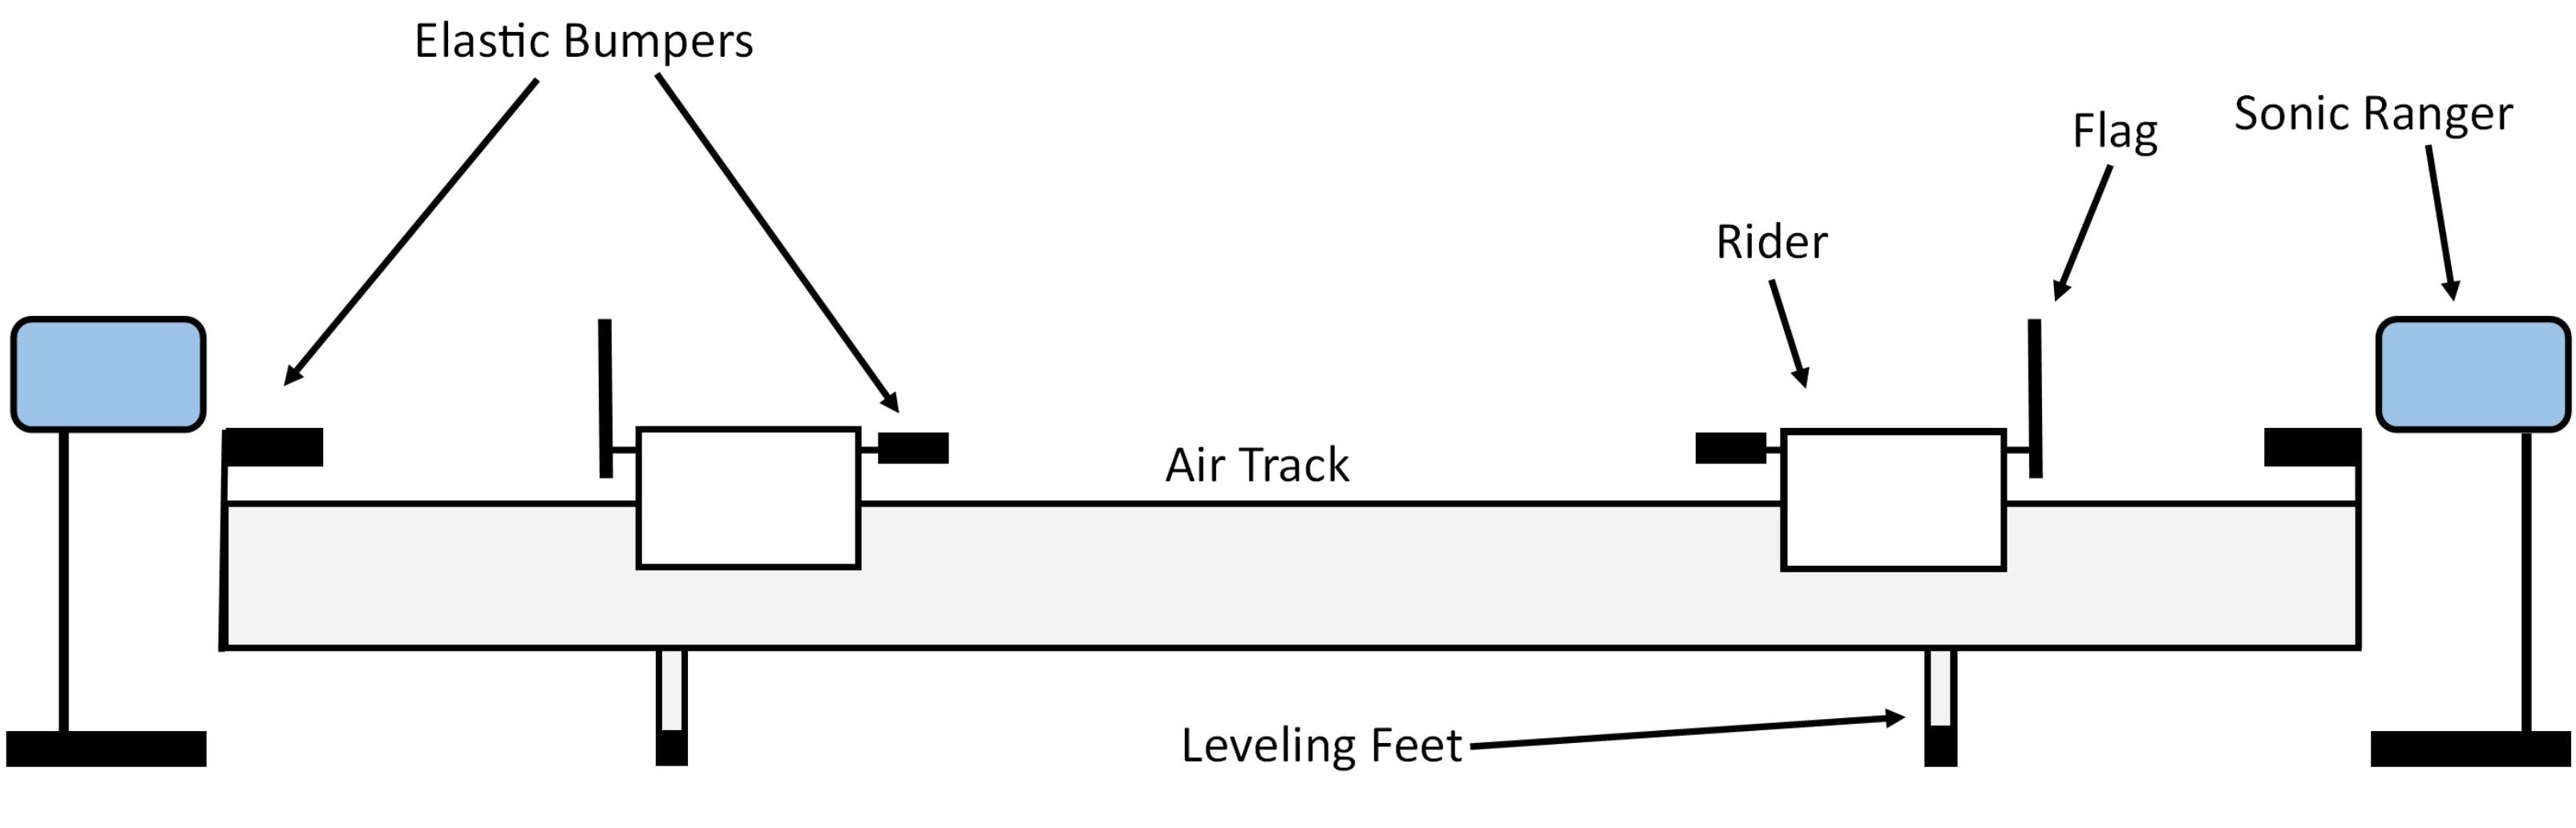
\includegraphics[width=0.9\textwidth]{Exp1-6/pic/image12.jpg}
    \caption{Schematic Diagram of the Air Track Setup}
    \label{fig:airtrack_p}
\end{center}
\end{figure}

In this experiment we use the computer in the lab to collect data. To log on, use the user name \textbf{student} and password \textbf{student}. On the desktop screen, click on the MOMENTUMLAB icon to load the software we use for this part of the lab.
\myskip

To begin taking data, single click on the \textbf{Start} button. As the data is being collected, the graph will dynamically display the current velocities of the two gliders. To stop taking data, single click on the \textbf{Stop} button. After analyzing the data, you may want to reset the graph by clicking on the menu \textbf{Experiment} $\rightarrow$ \textbf{Delete Last Data Run}.
\myskip

Make sure when exiting DataStudios, {\bf{do not}} save your current settings.
\subsubsection{Elastic Collision of Two Gliders}\label{sec:elastic}

In the air track experiment, we observe both elastic and inelastic collisions. The air track provides a steady airflow so that the gliders move along a layer of air and the effects of friction are negligible. We use bumpers and elastic rubber bands on the gliders to provide almost perfectly elastic collisions.\myskip

\begin{figure}[h]
    \begin{center}
        \begin{tikzpicture}[MyPerspective,scale=0.5,thick]
            \path (0.5,0,0);
            \pgfgetlastxy{\cylxx}{\cylxy}
            \path (0,0.5,0);
            \pgfgetlastxy{\cylyx}{\cylyy}
            \path (0,0,0.5);
            \pgfgetlastxy{\cylzx}{\cylzy}

            \pgfmathsetmacro{\cylt}{(\cylzy * \cylyx - \cylzx * \cylyy)/ (\cylzy * \cylxx - \cylzx * \cylxy)}
            \pgfmathsetmacro{\ang}{atan(\cylt)}
            \pgfmathsetmacro{\ct}{1/sqrt(1 + (\cylt)^2)}
            \pgfmathsetmacro{\st}{\cylt * \ct}

            \begin{scope}
                \draw (0.2,-1.8,-3) -- (-0.2,-1.8,-3) -- (-0.2,-1.8,0) -- (0.2,-1.8,0)  -- (0.2,-1.8,-2.5) -- (-0.1,-1.8,-2.5) -- (-0.1,-1.8,-2.6) -- (0.2,-1.8,-2.6) -- cycle;
                \draw (0,0,0) .. controls (0.8,0,2.3) and (-0.8,0,2.3) .. (0,0,0);
                \draw[fill=white] (-0.2,-1.8,0) -- (0.2,-1.8,0) -- (0.2,1.8,0) -- (-0.2,1.8,0) -- cycle;
                \draw[fill=gray] (0.2, -1.8, -2.5) -- (-0.1, -1.8, -2.5) -- (-0.1,1.8, -2.5) -- (0.2,1.8,-2.5) -- cycle;
                \draw[fill=white] (0.2,1.8,-3) -- (-0.2,1.8,-3) -- (-0.2,1.8,0) -- (0.2,1.8,0)  -- (0.2,1.8,-2.5) -- (-0.1,1.8,-2.5) -- (-0.1,1.8,-2.6) -- (0.2,1.8,-2.6) -- cycle;
            \end{scope}

            \begin{scope}[xshift=6cm]
                \draw (0,0) circle[x radius=0.5, y radius=0.5];
                \draw[fill=white] (0.47,0.03,-1.5) -- (0.47,0.03,0) -- (-0.47,0.03,0) -- (-0.47,0.03,-1.5) -- cycle;
                \draw[fill=white] (0.47,0.03,0) -- (0.47,0.03,-1.5) -- (0.47,-0.03,-1.5) -- (0.47,-0.03,0) -- cycle;
                \draw (-0.47,0.03,-1.5) -- (-0.47,-0.03,-1.5) -- (0.47,-0.03,-1.5);
                \draw (0,0,1.5) .. controls (0.8,0,3.8) and (-0.8,0,3.8) .. (0,0,1.5);
                \draw[fill=white] (\ct*0.5,\st*0.5,0) -- ++(0,0,1.5) arc[start angle=\ang,delta angle=180,radius=0.5] -- ++(0,0,-1.5) arc[start angle=\ang+180, delta angle=-180, radius=0.5];
                %\draw (
                %\draw[thick] (
            \end{scope}
        \end{tikzpicture}
    \end{center}
    \caption{Rubber Band Bumpers and Bumper Plates}
    \label{fig:bumpers}
\end{figure}

NOTE:  It is recommended that you ignore the error on masses, since they are so much smaller in comparison.

\begin{enumerate}
\item Insert an elastic rubber band bumper to the end of one glider (Figure \ref{fig:bumpers}), and insert a bumper plate to the end of the other glider.
\item Measure the masses of the gliders with these accessories on, without any additional mass first. Record the masses in your lab manual.
\item Put the two gliders onto the air track and make sure that the bumper plate is facing the rubber band bumper, and the two flags are facing the sonic rangers respectively, as shown in Figure \ref{fig:airtrack_p}.\label{st:start}
\item Click \textbf{Start} button to start collecting data and send the two gliders moving toward each other with an arbitrary velocity.
\item Record the velocities of the gliders right before collision $v_{1i}$, $v_{2i}$, and right after collision $v_{1f}$, $v_{2f}$.
\item Calculate the final velocities of the gliders from the $v_{1i}$ and $v_{2i}$ you measured with error (using equation \ref{eq:velocities}). Do your results agree with the final velocities you recorded using the sonic ranger?  \label{st:finish}
    %\item Repeat the experiment with some additional weights added to either of the glider. Does the theory still agree with experiment?
    %\item What would happen if the two gliders had exactly equal mass?
    %\item What would happen if you send a heavy glider to collide with a stationary light glider? Do we want this to happen?
    %\item What would happen if you placed the small glider stationary and send the large one on it? Why do we not want this to happen?

\enumeratext{Now we would like to study some special cases.}
  \item Discuss qualitatively what you expect to happen in the case of keeping one of the gliders stationary in the beginning, and sending the other glider to collide with this one.
  \item Repeat steps \ref{st:start}-\ref{st:finish} in this case. Record the velocities of the gliders right before the collision $v_{1i}$, $v_{2i}$, and right after collision $v_{1f}$, $v_{2f}$.
  \item Calculate the final velocities of the gliders from the $v_{1i}$ and $v_{2i}$ you measured with error (using equation \ref{eq:velocities}). Do your results agree with the final velocities you recorded using the sonic ranger? Do they agree with your expectations?

\enumeratext{Now add 2 additional weights to one of the gliders (make sure to put 1 weight on each side so that it is balanced and won't scratch the air track).}
  \item Put this heavier glider on the air track and keep it stationary. Discuss qualitatively what you expect to happen when you send the other glider with arbitrary velocity.
  \item  Send the other glider moving toward the heavier one with an arbitrary velocity. Record the velocities of the gliders right before collision $v_{1i}$, $v_{2i}$, and right after collision $v_{1f}$, $v_{2f}$.
  \item Calculate the final velocities of the gliders from the $v_{1i}$ and $v_{2i}$ you measured (using equation \ref{eq:velocities}). Do your results agree with the final velocities you recorded using the sonic ranger? Do they agree with your expectations? Don't worry about calculating error here.
  \item What would you expect to happen if the heavier glider is extremely massive, say with mass 100 times larger than the lighter one?
    %\item Calculate the final velocities of the gliders from the $v_{1i}$ and $v_{2i}$ data you measured from experiment. Do they agree with the final velocities you recorded using the sonic ranger?

\enumeratext{Repeat steps \ref{st:start}-\ref{st:finish} now with the lighter glider initially at rest, and send the heavier glider to collide with it. }
  \item Before starting, discuss qualitatively what you expect to happen in this case.
  \item Record the velocities of the gliders right before collision $v_{1i}$, $v_{2i}$, and right after collision $v_{1f}$, $v_{2f}$.
  \item Calculate the final velocities of the gliders from the $v_{1i}$ and $v_{2i}$ you measured (using equation \ref{eq:velocities}). Do your results agree with the final velocities you recorded using the sonic ranger? Do they agree with your expectations? Don't worry about calculating error here.
  \item What would you expect to happen if the heavier glider is extremely massive, say with mass 100 times larger than the lighter one?
    %\item Calculate the final velocities of the gliders from $v_{1i}$ and $v_{2i}$. Do they agree with the recorded final velocities?

\end{enumerate}

\subsubsection{Inelastic Collision of Two Gliders}

Replace the rubber band bumper and the bumper plate with a wax tube and a needle from the accessory box. The needle will stick into the wax tube and the two gliders will stick together after collision.
\begin{enumerate}
  \item First, keep one glider stationary and send the second glider toward the first one with some arbitrary velocity. Record the velocities of the gliders right before collision $v_{1i}$, $v_{2i}$, and right after collision $v_{1f}$, $v_{2f}$.
  \item Calculate the combined velocity of the two gliders after collision from the $v_{1i}$ and $v_{2i}$ you measured from experiment. Does it agree with the velocity you recorded using the sonic ranger? Don't worry about calculating error here.
  \item Repeat  steps 1-2 with both gliders moving towards each other. Try a few times to find initial velocities such that both gliders come to rest after collision.
  \item What is the ratio of their velocities when the final velocity is zero? Is it what you expect?
%\item Compare the experimental velocity ratio to a theoretical prediction from the masses of the gliders
%\item After bouncing off the ends, do the two gliders meet again at the position from which they started?  Explain why or why not!
\end{enumerate}

\subsection{The Ballistic Pendulum}
\emph{Safety remark}: Do not have the projectile launcher loaded while you are taking measurements or setting up. Remember to wear the safety goggles when you are actually doing the experiment.\myskip

In this experiment, we will measure the velocity of a projectile from a spring-loaded launcher and use it to predict the behavior of a pendulum with which it is colliding. The components are shown in the following diagram:

\begin{figure}[h]
    \begin{center}
        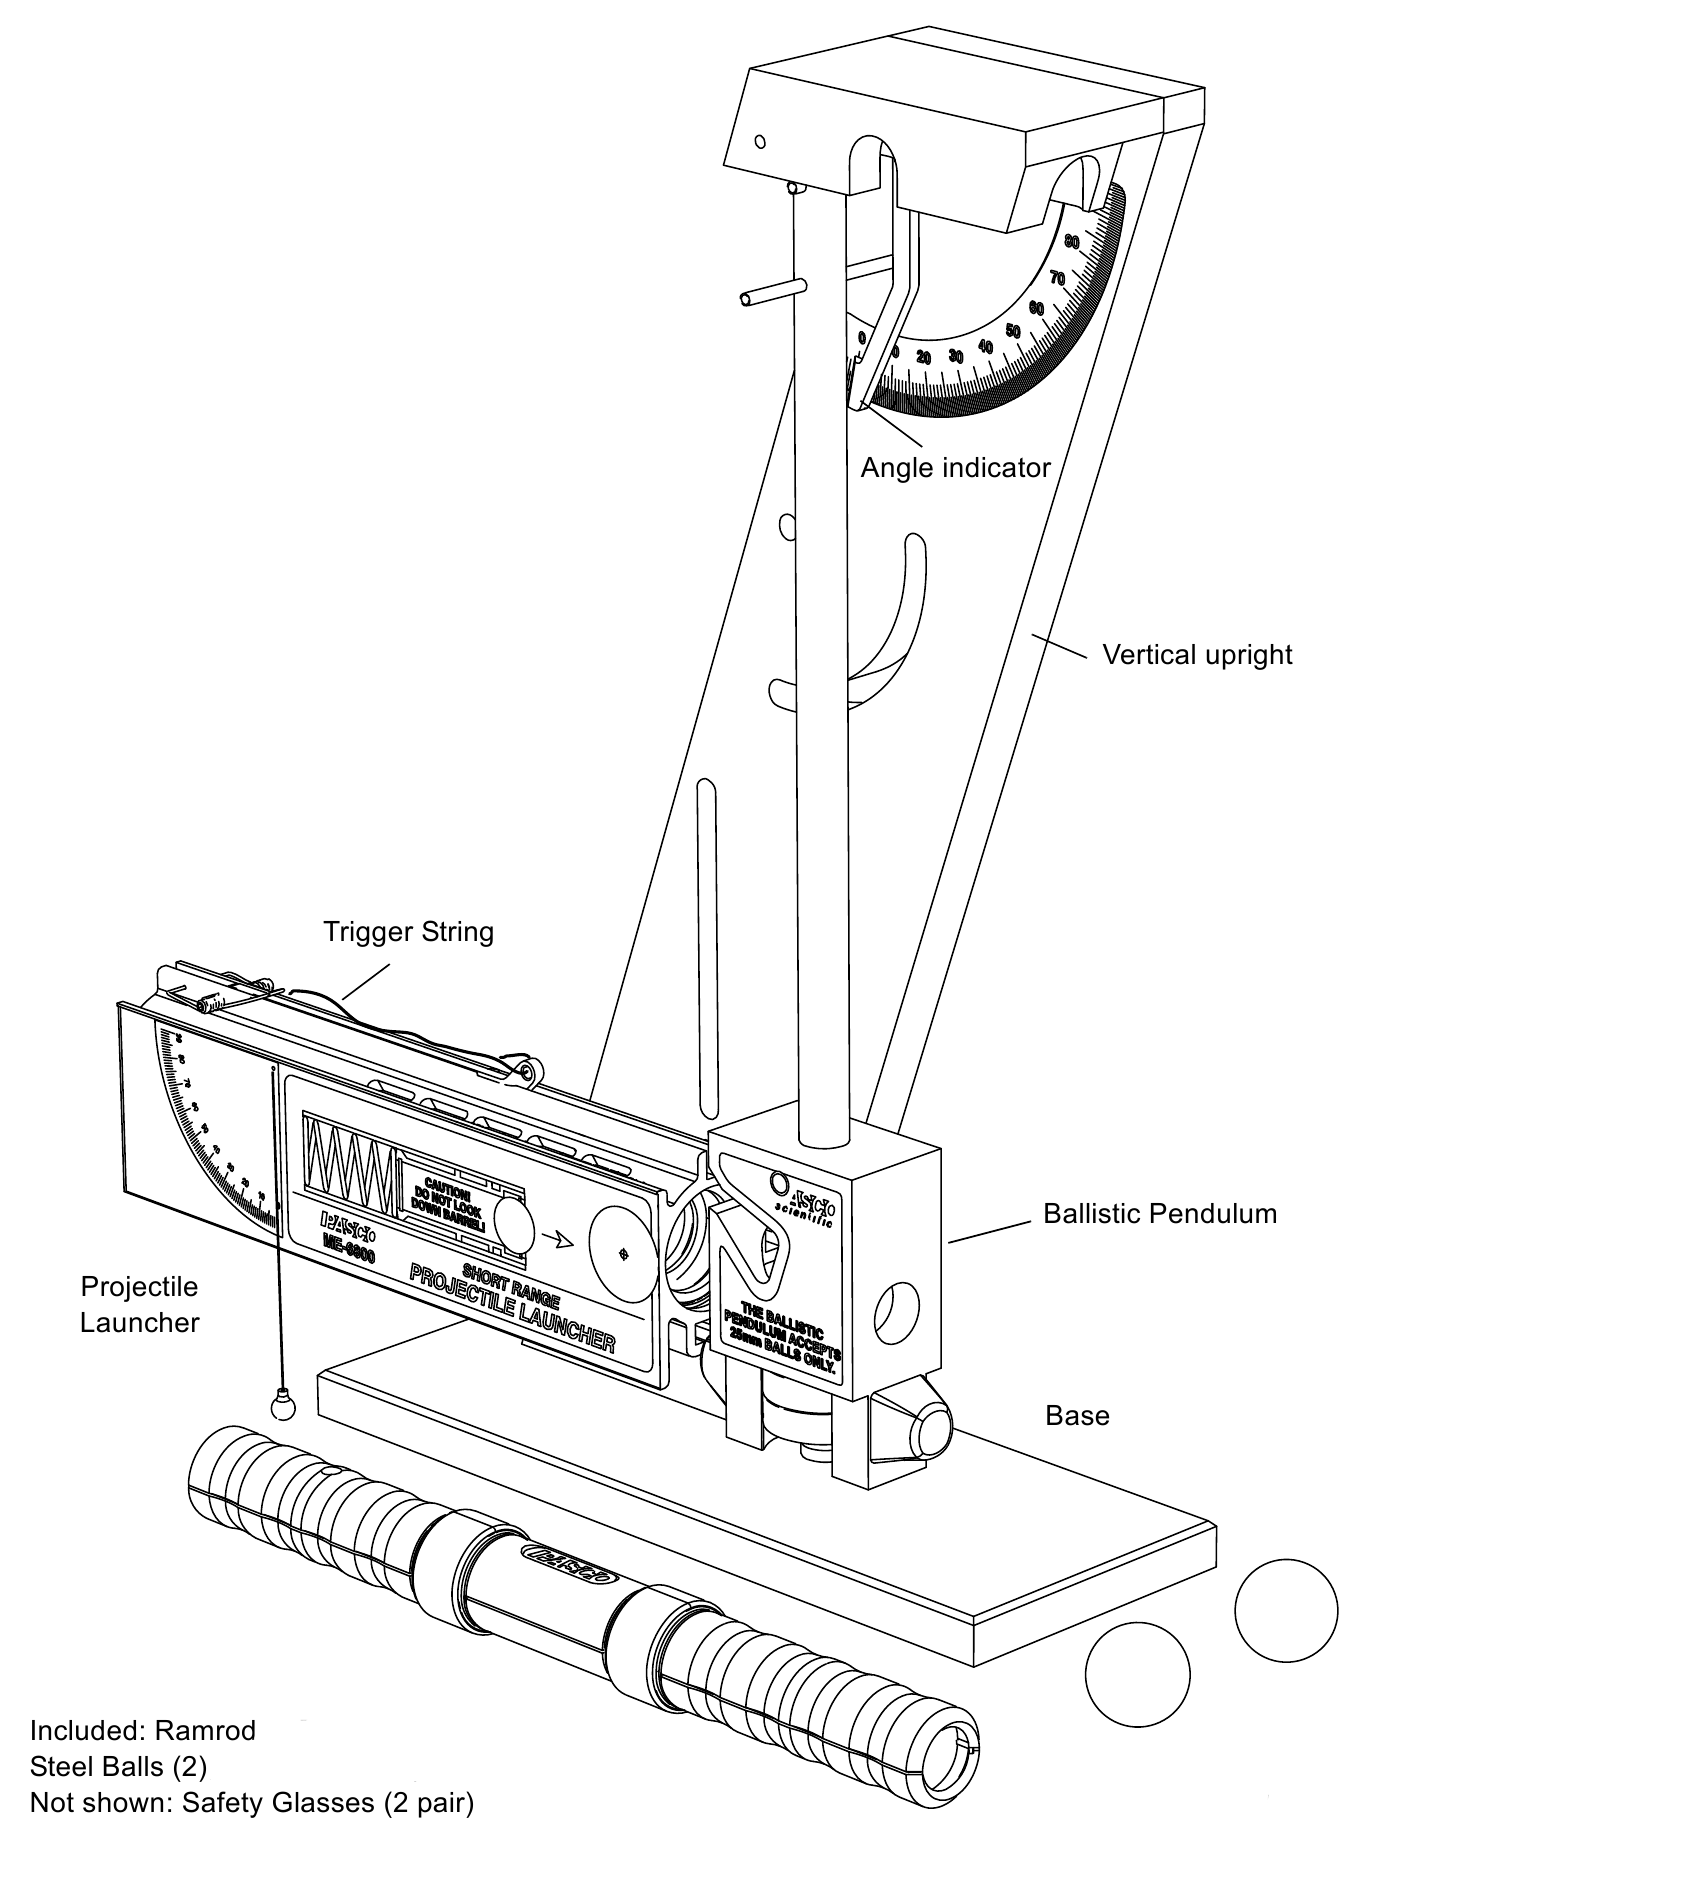
\includegraphics[height=0.6\textheight]{./Exp1-6/pic/image3.png}
    \end{center}
    \caption{Ballistic Pendulum}
    \label{fig:ballistic}
\end{figure}

%TODO: Add a diagram

\begin{itemize}
    \item \textbf{Launcher} - We will be using a spring-loaded launcher to propel our projectile.  There are 3 different velocity settings, i.e.\ three different positions to which you can compress the spring.  We assume that for a single spring position, the projectile will show very little variability in its velocity between launchings (you can convince yourself of this in the next section!).
    \item \textbf{Pendulum} - The pendulum consists of a rigid rod with a cup (and some brass weights) at one end.  The cup has a latch which will trap the ball inside upon impact.  The rod has a non-negligible mass, but we will assume that our pendulum is a simple pendulum, with all weight concentrated at the end.
    %\item \textbf{Photogate Timers} - To measure the initial velocity of our projectile, we will use two photogate timers.  These send a signal whenever a solid object passes through their beam.  Note that the construction of our pendulum does not allow us to measure the projectile's velocity \textit{in situ} - we must measure the projectile's velocity with the pendulum moved away, and then assume a similar velocity for subsequent trials.  Because our launcher gives highly repeatable results, this is not a bad assumption.
\end{itemize}

\subsubsection{Measuring $\theta$}\label{subsubsec:theta}

First, make sure that that the launcher is attached to the bottom set of slots, as shown in the above diagram. The plumb bob at the end of the launcher indicates the angle of inclination of the launcher.  Arrange the launcher so that it lays level, and then load the metal ball into the launcher, compressing the spring to one of the 3 possible load positions. Write down the corresponding quoted velocity of the ball out of the launcher.  Note that during the loading, the pendulum can be clipped to the 90 degrees position so that it stays out of the way. \myskip

Once the metal ball is loaded, bring the pendulum down.  The black angle indicator should be in position so that it is pushed upward as the pendulum swings forward.  It is designed to stick to the position to which the pendulum pushes it, without slipping backward due to gravity.  If you find that the indicator does slip backward, a rubber band can be used to hold it in place. \myskip

Because the base plate may not rest on a perfectly level surface, the angle indicator at the top of the pendulum may not point to zero even when the pendulum is pointing straight down.  Therefore you should first record the initial (small) angle of the pendulum, and then record the final angle of the pendulum, subtracting the two to find the total angle swung through by the pendulum.\myskip

You are ready to launch.  With the pendulum in position, and the whole setup pointed toward a safe place (away from your fellow physicists!), pull the yellow cord, which releases the catch on the launcher and launches your metal ball.
\begin{enumerate}
\item Record the resulting angle of the pendulum, and repeat this procedure 5 times, recording the final angle $\theta_\text{f}$ each time.
\item Find the average final angle $\theta_\text{f,ave}$ with error. Error can be found using the 2/3 method.
\end{enumerate}


\subsubsection{Other Measurements}

In order to calculate the initial velocity, we must also know the masses of the ball and the pendulum, as well as the pendulum's length. In order to measure these quantities, you can unscrew the pendulum and take it off from the base. Measure all of these using the electric scale and your ruler, and use them (along with the angle swept out by the pendulum) to make an estimation of the metal ball's initial velocity.\myskip

\begin{enumerate}
    \item Calculate the initial ball velocity $v_{i}$ with error found by propagating uncertainties in $\theta$. You can ignore all other errors in your velocity expression and propagate only through $\theta$. To do so, you will need to find the uncertainty in $\cos(\theta)$ which can be found as follows:
\begin{gather}
\sigma_{\cos(\theta)} = \Bigg{|}\frac{\cos(\theta + \sigma_\theta) - \cos(\theta - \sigma_\theta)}{2} \Bigg{|}
\end{gather}
Note, the uncertainty in $\theta$ comes from the 2/3 method as discussed in 3.2.1.2.
\item Does your calculated initial ball velocity agree with what is labelled on the pendulum within error?
\item Discuss the major sources of error in determining the initial ball velocity.
    \item Repeat steps in \ref{subsubsec:theta} with a different compression for the spring, i.e.\ different initial velocity. Which of your result agrees better with the labelled value? %You can have at most 3 different initial velocities. Compare your experimental results with the labelled values on the pendulum, which one agrees best?
    \item In making our prediction, we assumed a simple pendulum (i.e.\ one with all mass concentrated at the end).  Were you to make a more careful calculation, what steps in our derivation would require modification?
\end{enumerate}

\section{Lab Preparation Examples}
{\bf{Note: Suggested prelab questions are in bold. These will help will conceptual understanding of the laboratory experiments.}}
\\
\\
\noindent\underline{Propagation of Uncertainty}:\myskip

{\bf{1. Given $a = 1.5 \pm 0.5\, \textrm{m}$ and $b = 3.0 \pm 0.6\, \textrm{m}$ what is $a/b$?}}\myskip

\noindent\underline{Ballistic Pendulum}:\myskip

2. You measure the following values for the pendulum experiment:
\begin{table}[h]
  \centering
  \begin{tabular}{|c|c|c|c|}
    \hline
    $\theta$&$R$&$m$&$M$\\
    \hline
    $25^\circ$ & $30\,\mathrm{cm}$ & $30\,\textrm{g}$ & $300\,\textrm{g}$\\
    \hline
  \end{tabular}
\end{table}

What is your predicted value for $v_0$? (Answer: $8.16\,\mathrm{m/s}$)\myskip

\noindent\underline{Conversion m/s, km/h and miles/h}: \myskip

{\bf{4. What is $1\, \textrm{m/s}$ in km/h?}}
\myskip

5. How many miles/h is the speed of $200\,\textrm{km/s}$?\myskip


\noindent\underline{Air track}:\myskip

6. In the elastic collision, the gliders weigh $m = 100\,\textrm{g}$ and $M = 250\textrm{g}$. The heavier glider is stationary, whereas the lighter one initially travels towards it with velocity $v_{1i} = 1.5\,\mathrm{m/s}$. What is the expected value for $v_{1f}$ and $v_{2f}$? (Answer: $-0.64\,\mathrm{m/s}$ and $0.86\,\mathrm{m/s}$ respectively)\myskip

{\bf{7. In the inelastic collision, the gliders weigh $m = 100\,\textrm{g}$ and $M = 250\textrm{g}$. The heavier glider is stationary, whereas the lighter one initially travels towards it with velocity $v_{1i} = 1.5\,\mathrm{m/s}$. What is the expected value for $v_{1f}$ and $v_{2f}$? (Answer: $0.43\,\mathrm{m/s}$ for both)}}
\myskip

\noindent\underline{Explanations}:\myskip

{\bf{8. You are sitting in a car of mass $M$. Another car with mass $m = 500\,\textrm{kg}$ crashes into you with a relative velocity of $10\,\textrm{m/s}$. Explain in a few sentences (and maybe equations) why you feel less impact if your car has $M = 2000\,\textrm{kg}$ as if your car has only $M = 500\,\textrm{kg}$? }}
